\section*{Introduction}

A function can be thought of as a \emph{meat grinder}.\footnote{
    My apologies to vegetarians and vegans.
}
You put chunks of beef into a meat grinder (the \emph{input}),
and ground hamburger comes out (the \emph{output}). 

\begin{center}
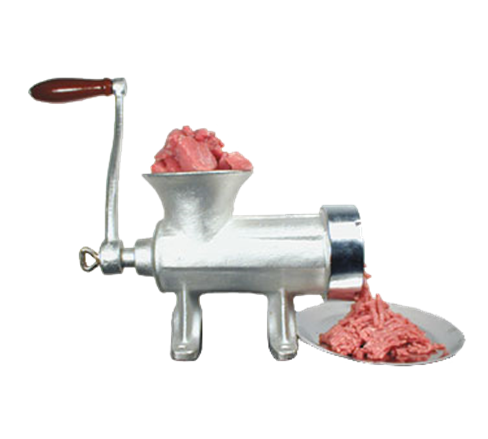
\includegraphics[width=1.5in]{../../common/images/meat-grinder.png} 
\end{center}

\begin{center}
\(
    \text{chunks of beef}
    \Longrightarrow
    \text{meat-grinder-function}
    \Longrightarrow
    \text{ground hamburger}
\)
\end{center}

Similarly,
in math a function has \emph{inputs} and \emph{outputs}.
We usually use $x$ for the inputs and $y$ as the outputs.
You put $x$'s into a function, $f(x)$,
and $y$'s come out.
Think of the $x$'s as the chunks of beef
and the $y$'s as the ground hamburger.
\begin{center}
\(
    x
    \Longrightarrow
    f
    \Longrightarrow
    y
\)
\end{center}

You could ``daisy chain'' two meat grinders---when 
you take the output of one and push it into
a second one.
The two griders act as a  
\emph{single, bigger meat grinder} which takes chunks of beef
as an input and creates 
{\bfseries\itshape ultra-ground beef} as an output.

\begin{center}
    \fbox{
        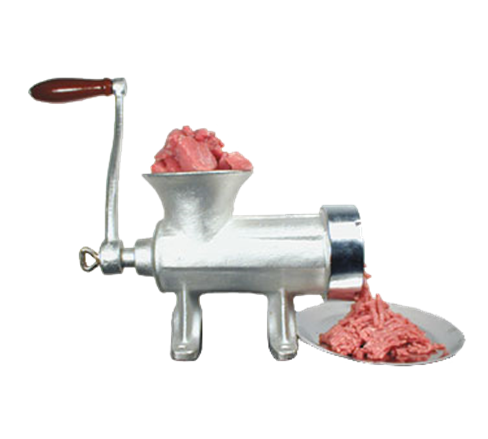
\includegraphics[width=1.5in]{../../common/images/meat-grinder.png}
        \begin{minipage}[b][1.25in][c]{0.5in}
            \centering\HUGE\bfseries
            $\nearrow$
        \end{minipage}
        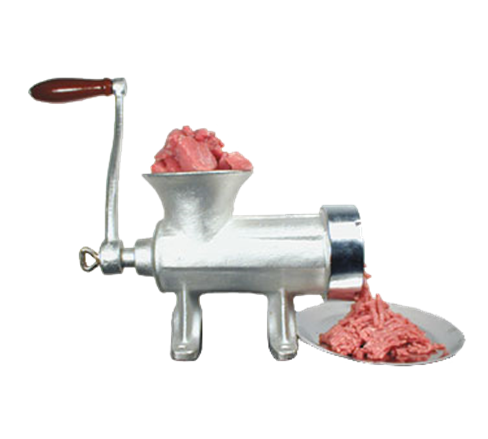
\includegraphics[width=1.5in]{../../common/images/meat-grinder.png} 
    }
\end{center}
To emphasize that the two grinders work together, 
we could draw it like this 
\begin{center}
    \fbox{
        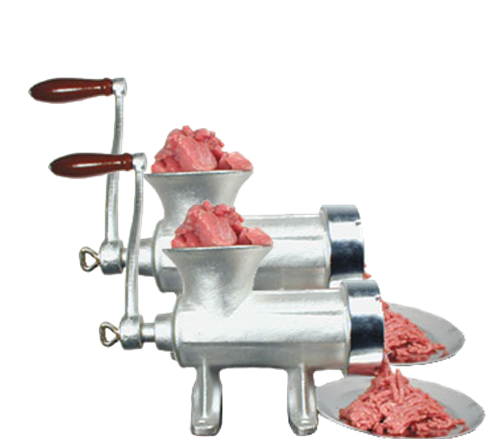
\includegraphics[width=1.5in]{../../common/images/composite-meat-grinder.png} 
    }
\end{center}
This is called ``composing''. 
We have composed two meat grinders
into a single, bigger grinder in the box that is called 
a ``composite grinder''.

In math, when you do this to functions,
you are ``composing'' the two functions
into \emph{single, bigger functions}.
We call these ``composite functions''.

\begin{center}
\vspace{1em}
\(
    x
    \Longrightarrow
\)
\fbox{
    \(
        f
        \Longrightarrow
        g
    \)
}
\(
    \Longrightarrow
    y
\)
\vspace{1em}
\end{center}

That thing in the box is a composite function which is composed of $f$ and $g$.
The mathematical notion for a composite of two functions is a small circle
$g\circ f$ is a single, bigger composite function. We will usually write it with parentheses around it:
$(g\circ f)$.

This can be confusing, because it is very abstract.
So let's look at an example.

\begin{myExample}{An example of composing two functions.}
    Consider these functions:
    \begin{align*}
        f(x) &= 2x + 3 \\
        g(x) &= -x^2 + 5
    \end{align*}
    You already know how to evaluate them at (say) $x=1$:
    \begin{align*}
        f(1) &= 2(1) + 3   = 2+3    = 5\\
        g(1) &= -(1)^2 + 5 = -1 + 5 = 4
    \end{align*}
    When we \emph{compose} functions, 
    we evaluate one of them and take the {\bfseries\itshape output} and pass it 
    into the other one.
    Suppose we evalute $g$ first and then pass its output to $f$.
    We write this composite function as $f\circ g$ (which looks {\bfseries\itshape backwards}!):
    \vskip1em
    Evaluating the composite function $(f\circ g)$ with an input $1$ is written like this: $(f\circ g)(1)$, and here is how to calculate the output.
    \begin{enumerate}
        \item Pass the input to the ``nearest'' function. In this case, we pass $1$ to $g$.
        \item Calculate the output of that function. In this case, $g(1) = 4$.
        \item Pass that output to the next function. In this case, we pass $4$ to $f$.
        \item Calculate the output from that function. In this case, $f(4) = 2(4) + 3 = 8+3 = 11$.
        \item That result is the output of the composite function. In other words, $(f\circ g)(1) = 11$.
    \end{enumerate}
\end{myExample}


\begin{center}
    \begin{tcolorbox}[width=4in]
        {\bfseries\itshape Warning:}
        The order of composite functions makes a difference. 
        $(f \circ g)$ 
        and
        $(g \circ f)$ 
        are {\bfseries\itshape not} the same.
    \end{tcolorbox}
\end{center}